%%%%%%%%%%%%%%%%%%%%%%%%%%%%%%%%%%%%%%%%%%%%%%%%%%%%%%%%%%%%%%%%%%%%%%%%%
% Deep Reinforcement Learning for EV Routing Optimization
% Streamlined Presentation - Focus on Figures
% Authors: Salem Fradi & Dhia Elhak Ezzeddini
%%%%%%%%%%%%%%%%%%%%%%%%%%%%%%%%%%%%%%%%%%%%%%%%%%%%%%%%%%%%%%%%%%%%%%%%%

\documentclass[aspectratio=169,11pt]{beamer}

%-------------------------------------------------------------------------
% THEME AND COLORS
%-------------------------------------------------------------------------
\usetheme{Madrid}
\usecolortheme{whale}

\definecolor{primaryblue}{RGB}{0,84,147}
\definecolor{secondaryblue}{RGB}{0,119,182}
\definecolor{accentgreen}{RGB}{0,150,136}
\definecolor{lightgray}{RGB}{245,245,245}
\definecolor{darkgray}{RGB}{60,60,60}

\setbeamercolor{palette primary}{bg=primaryblue,fg=white}
\setbeamercolor{palette secondary}{bg=secondaryblue,fg=white}
\setbeamercolor{palette tertiary}{bg=primaryblue,fg=white}
\setbeamercolor{structure}{fg=primaryblue}
\setbeamercolor{title}{fg=white,bg=primaryblue}
\setbeamercolor{frametitle}{fg=white,bg=primaryblue}
\setbeamercolor{block title}{bg=primaryblue,fg=white}
\setbeamercolor{block body}{bg=lightgray,fg=darkgray}
\setbeamercolor{block title alerted}{bg=red!70!black,fg=white}
\setbeamercolor{block title example}{bg=accentgreen,fg=white}

%-------------------------------------------------------------------------
% PACKAGES
%-------------------------------------------------------------------------
\usepackage[utf8]{inputenc}
\usepackage[T1]{fontenc}
\usepackage{amsmath,amsfonts,amssymb}
\usepackage{graphicx}
\usepackage{booktabs}
\usepackage{tikz}
\usepackage{pgfplots}
\usepackage{xcolor}
\usepackage{hyperref}
\usepackage{caption}
\usepackage{subcaption}
\usepackage{array}
\usepackage{multirow}
\usepackage{fontawesome5}
\usepackage{pifont}

\usetikzlibrary{shapes,arrows,positioning,calc,decorations.pathreplacing,fit,backgrounds}
\pgfplotsset{compat=1.17}

%-------------------------------------------------------------------------
% CUSTOM COMMANDS
%-------------------------------------------------------------------------
\newcommand{\cmark}{\ding{51}}
\newcommand{\xmark}{\ding{55}}
\newcommand{\highlight}[1]{\textcolor{accentgreen}{\textbf{#1}}}

%-------------------------------------------------------------------------
% FOOTER
%-------------------------------------------------------------------------
\setbeamertemplate{navigation symbols}{}
\setbeamertemplate{footline}{
    \leavevmode%
    \hbox{%
        \begin{beamercolorbox}[wd=.333333\paperwidth,ht=2.25ex,dp=1ex,center]{author in head/foot}%
            \usebeamerfont{author in head/foot}\insertshortauthor
        \end{beamercolorbox}%
        \begin{beamercolorbox}[wd=.333333\paperwidth,ht=2.25ex,dp=1ex,center]{title in head/foot}%
            \usebeamerfont{title in head/foot}\insertshorttitle
        \end{beamercolorbox}%
        \begin{beamercolorbox}[wd=.333333\paperwidth,ht=2.25ex,dp=1ex,right]{date in head/foot}%
            \usebeamerfont{date in head/foot}\insertshortdate{}\hspace*{2em}
            \insertframenumber{} / \inserttotalframenumber\hspace*{2ex}
        \end{beamercolorbox}}%
    \vskip0pt%
}

%-------------------------------------------------------------------------
% TITLE INFORMATION
%-------------------------------------------------------------------------
\title[DRL for EV Routing]{Deep Reinforcement Learning for\\Electric Vehicle Routing Optimization}
\subtitle{Energy-Minimizing Electric Vehicle Routing Problem (EM-EVRP)}
\author[D. Ezzeddini \& S. Fradi]{Dhia Elhak Ezzeddini \and Salem Fradi}
\institute[Sup'Com]{
    Higher School of Communication of Tunis -- Carthage University\\[0.2cm]
    \textbf{Supervisor:} Dr. Ferdaoues Chaabane \quad \textbf{Host:} Sagemcom
}
\date{Academic Year 2025--2026}

\graphicspath{{../docs/figures/}{../images/}}

%=========================================================================
\begin{document}
%=========================================================================

%-------------------------------------------------------------------------
\begin{frame}[plain]
    \titlepage
\end{frame}

%-------------------------------------------------------------------------
\begin{frame}{Outline}
    \tableofcontents[hideallsubsections]
\end{frame}

%=========================================================================
\section{Introduction}
%=========================================================================

%-------------------------------------------------------------------------
\begin{frame}{Context: EV Adoption \& Logistics Challenges}
    \begin{columns}[T]
        \begin{column}{0.48\textwidth}
            \begin{block}{Global Trends}
                \begin{itemize}
                    \item 14M+ EVs sold in 2023
                    \item 40M+ expected by 2030
                    \item Corporate sustainability push
                \end{itemize}
            \end{block}

            \begin{alertblock}{Core Challenge}
                Limited range \& sparse charging $\Rightarrow$ \textbf{smart routing required}
            \end{alertblock}
        \end{column}
        \begin{column}{0.48\textwidth}
            \begin{center}
                \begin{tikzpicture}[scale=0.7,
                    challenge/.style={rectangle, rounded corners, draw=primaryblue, fill=lightgray,
                                     text width=2.2cm, minimum height=0.9cm, align=center, font=\scriptsize}
                ]
                    \node[ellipse, draw=primaryblue, fill=primaryblue!20, text width=1.8cm,
                          align=center, font=\bfseries\scriptsize] (center) {EV\\Challenges};
                    \node[challenge] (range) at (-2.5,1.5) {\faIcon{battery-half}\\Limited Range};
                    \node[challenge] (charge) at (-2.5,-1.5) {\faIcon{charging-station}\\Sparse Charging};
                    \node[challenge] (energy) at (2.5,1.5) {\faIcon{bolt}\\Variable Energy};
                    \node[challenge] (plan) at (2.5,-1.5) {\faIcon{route}\\Complex Routing};
                    \draw[->, thick, primaryblue] (center) -- (range);
                    \draw[->, thick, primaryblue] (center) -- (charge);
                    \draw[->, thick, primaryblue] (center) -- (energy);
                    \draw[->, thick, primaryblue] (center) -- (plan);
                \end{tikzpicture}
            \end{center}
        \end{column}
    \end{columns}

    \vspace{0.4cm}
    \begin{exampleblock}{Our Contribution}
        \centering
        End-to-end DRL solution + physics-based energy model + real-world deployment
    \end{exampleblock}
\end{frame}

%=========================================================================
\section{Problem Statement}
%=========================================================================

%-------------------------------------------------------------------------
\begin{frame}{Energy-Minimizing EVRP (EM-EVRP)}
    \begin{columns}[T]
        \begin{column}{0.42\textwidth}
            \begin{block}{Objective}
                Minimize \textbf{total energy consumption} while serving all customers
            \end{block}

            \vspace{0.3cm}
            \textbf{Key Constraints:}
            \begin{itemize}
                \item Each customer visited once
                \item Vehicle capacity limits
                \item Battery SOC $\geq 0$ always
                \item Optional charging stops
            \end{itemize}

            \vspace{0.3cm}
            \begin{alertblock}{NP-Hard}
                Exact methods don't scale!
            \end{alertblock}
        \end{column}
        \begin{column}{0.55\textwidth}
            \begin{center}
                \begin{tikzpicture}[scale=0.85]
                    % Depot
                    \node[rectangle, draw=red, fill=red!30, minimum size=0.7cm] (depot) at (0,0) {\faIcon{warehouse}};
                    \node[below=0.1cm of depot, font=\scriptsize] {Depot};

                    % Charging stations
                    \node[circle, draw=accentgreen, fill=accentgreen!30, minimum size=0.6cm] (cs1) at (-2.5,2.5) {\faIcon{plug}};
                    \node[circle, draw=accentgreen, fill=accentgreen!30, minimum size=0.6cm] (cs2) at (2.5,-2) {\faIcon{plug}};

                    % Customers
                    \node[circle, draw=primaryblue, fill=primaryblue!30, minimum size=0.5cm] (c1) at (-2,-1.2) {};
                    \node[circle, draw=primaryblue, fill=primaryblue!30, minimum size=0.5cm] (c2) at (1.2,2.5) {};
                    \node[circle, draw=primaryblue, fill=primaryblue!30, minimum size=0.5cm] (c3) at (3,1.2) {};
                    \node[circle, draw=primaryblue, fill=primaryblue!30, minimum size=0.5cm] (c4) at (-2.5,-2.5) {};
                    \node[circle, draw=primaryblue, fill=primaryblue!30, minimum size=0.5cm] (c5) at (0.8,-3) {};

                    % Route 1
                    \draw[->, very thick, red!70] (depot) -- (c1);
                    \draw[->, very thick, red!70] (c1) -- (c4);
                    \draw[->, very thick, red!70] (c4) -- (cs1);
                    \draw[->, very thick, red!70] (cs1) -- (c2);
                    \draw[->, very thick, red!70] (c2) -- (depot);

                    % Route 2
                    \draw[->, very thick, blue!70, dashed] (depot) -- (c3);
                    \draw[->, very thick, blue!70, dashed] (c3) -- (c5);
                    \draw[->, very thick, blue!70, dashed] (c5) -- (cs2);
                    \draw[->, very thick, blue!70, dashed] (cs2) -- (depot);

                    % Legend
                    \node[font=\scriptsize] at (0, -4) {Multi-vehicle routes with charging stops};
                \end{tikzpicture}
            \end{center}
        \end{column}
    \end{columns}
\end{frame}

%-------------------------------------------------------------------------
\begin{frame}{Why Minimize Energy Instead of Distance?}
    \begin{center}
        \fbox{\parbox{0.8\textwidth}{\centering
            \textbf{Key Insight:} Shortest path $\neq$ most energy-efficient path!\\[0.2cm]
            A longer downhill route may use \textit{less} energy than a shorter uphill one.
        }}
    \end{center}

    \vspace{0.5cm}
    \begin{columns}[T]
        \begin{column}{0.48\textwidth}
            \textbf{Energy depends on:}
            \begin{itemize}
                \item \highlight{Vehicle load} (heavier = more energy)
                \item \highlight{Road gradient} (uphill vs downhill)
                \item \highlight{Speed profile} \& aerodynamic drag
                \item \highlight{Regenerative braking}
            \end{itemize}
        \end{column}
        \begin{column}{0.48\textwidth}
            \begin{exampleblock}{Benefits of Energy Optimization}
                \begin{itemize}
                    \item Extended range per charge
                    \item Fewer charging stops
                    \item Lower operational costs
                    \item Reduced battery degradation
                \end{itemize}
            \end{exampleblock}
        \end{column}
    \end{columns}
\end{frame}

%=========================================================================
\section{Energy Consumption Model}
%=========================================================================

%-------------------------------------------------------------------------
\begin{frame}{Physics-Based Energy Model}
    \begin{block}{Mechanical Power Required on Arc $(i,j)$}
        \[
        P_{ij} = \underbrace{\frac{1}{2} C_d \rho A v_{ij}^2}_{\text{Aerodynamic drag}} +
                 \underbrace{m_{ij} g \sin\alpha_{ij}}_{\text{Gravitational}} +
                 \underbrace{m_{ij} g C_r \cos\alpha_{ij}}_{\text{Rolling resistance}}
        \]
    \end{block}

    \begin{columns}[T]
        \begin{column}{0.48\textwidth}
            \begin{block}{Energy with Efficiency}
                \[
                E_{ij} = \begin{cases}
                    \phi_d \varphi_d P_{ij} t_{ij} & P_{ij} \geq 0 \\
                    \phi_r \varphi_r P_{ij} t_{ij} & P_{ij} < 0
                \end{cases}
                \]
                \small Negative power = regeneration!
            \end{block}
        \end{column}
        \begin{column}{0.48\textwidth}
            \begin{block}{Key Parameters}
                \small
                \begin{tabular}{cl}
                    $m_{ij}$ & Vehicle + cargo mass \\
                    $\alpha_{ij}$ & Road slope angle \\
                    $C_d, C_r$ & Drag coefficients \\
                    $\phi, \varphi$ & Efficiencies
                \end{tabular}
            \end{block}
        \end{column}
    \end{columns}

    \vspace{0.3cm}
    \begin{center}
        \textbf{Objective:} $\displaystyle\min \sum_{k} \sum_{(i,j)} E_{ij} \cdot x_{ijk}$
    \end{center}
\end{frame}

%=========================================================================
\section{Data Generation \& System Architecture}
%=========================================================================

%-------------------------------------------------------------------------
\begin{frame}{Training Data Generation}
    \begin{columns}[T]
        \begin{column}{0.45\textwidth}
            \begin{block}{Synthetic Data}
                \begin{itemize}
                    \item Random coordinates on $100 \times 100$ grid
                    \item Random elevations for slopes
                    \item Random customer demands
                    \item Pairwise distances \& energy costs
                \end{itemize}
            \end{block}

            \begin{block}{Dataset Size}
                \begin{tabular}{ll}
                    Training & 1,280,000 \\
                    Validation & 10,000 \\
                    Batch size & 1,024
                \end{tabular}
            \end{block}
        \end{column}
        \begin{column}{0.52\textwidth}
            \begin{center}
                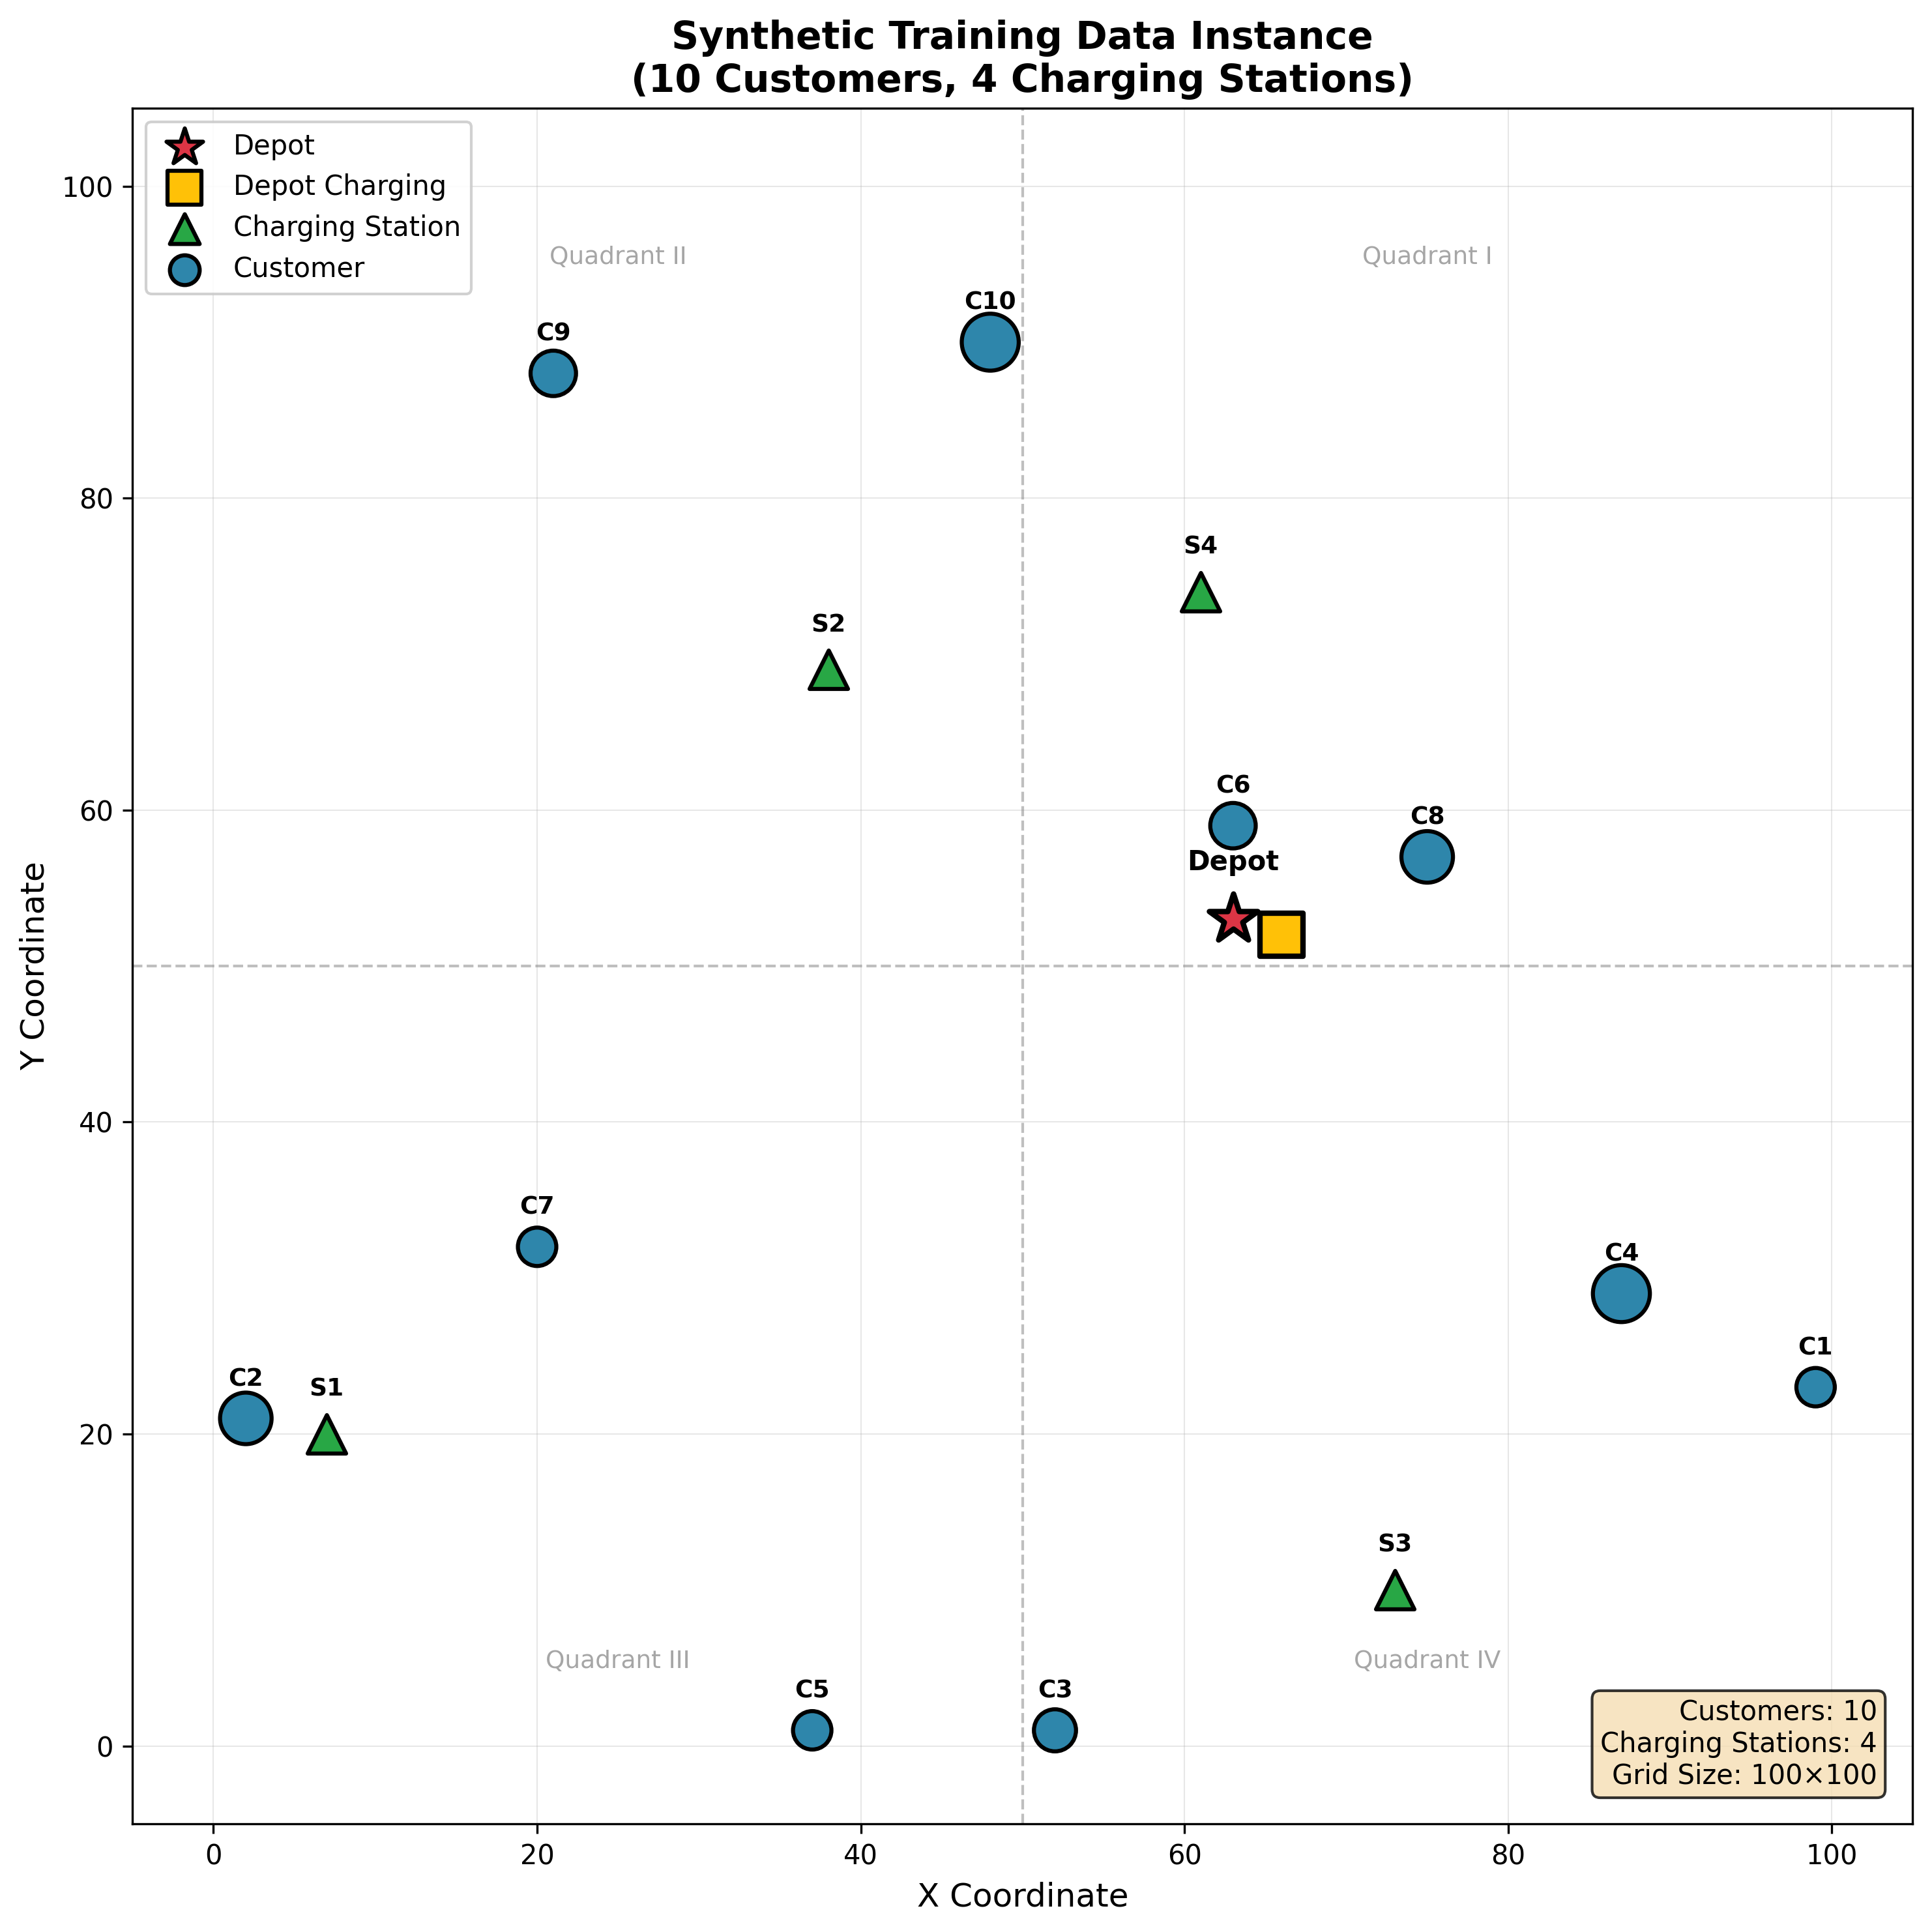
\includegraphics[width=\textwidth]{synthetic_training_data.png}
            \end{center}
            \small\centering Sample training instance
        \end{column}
    \end{columns}
\end{frame}

%-------------------------------------------------------------------------
\begin{frame}{End-to-End System Pipeline}
    \begin{center}
        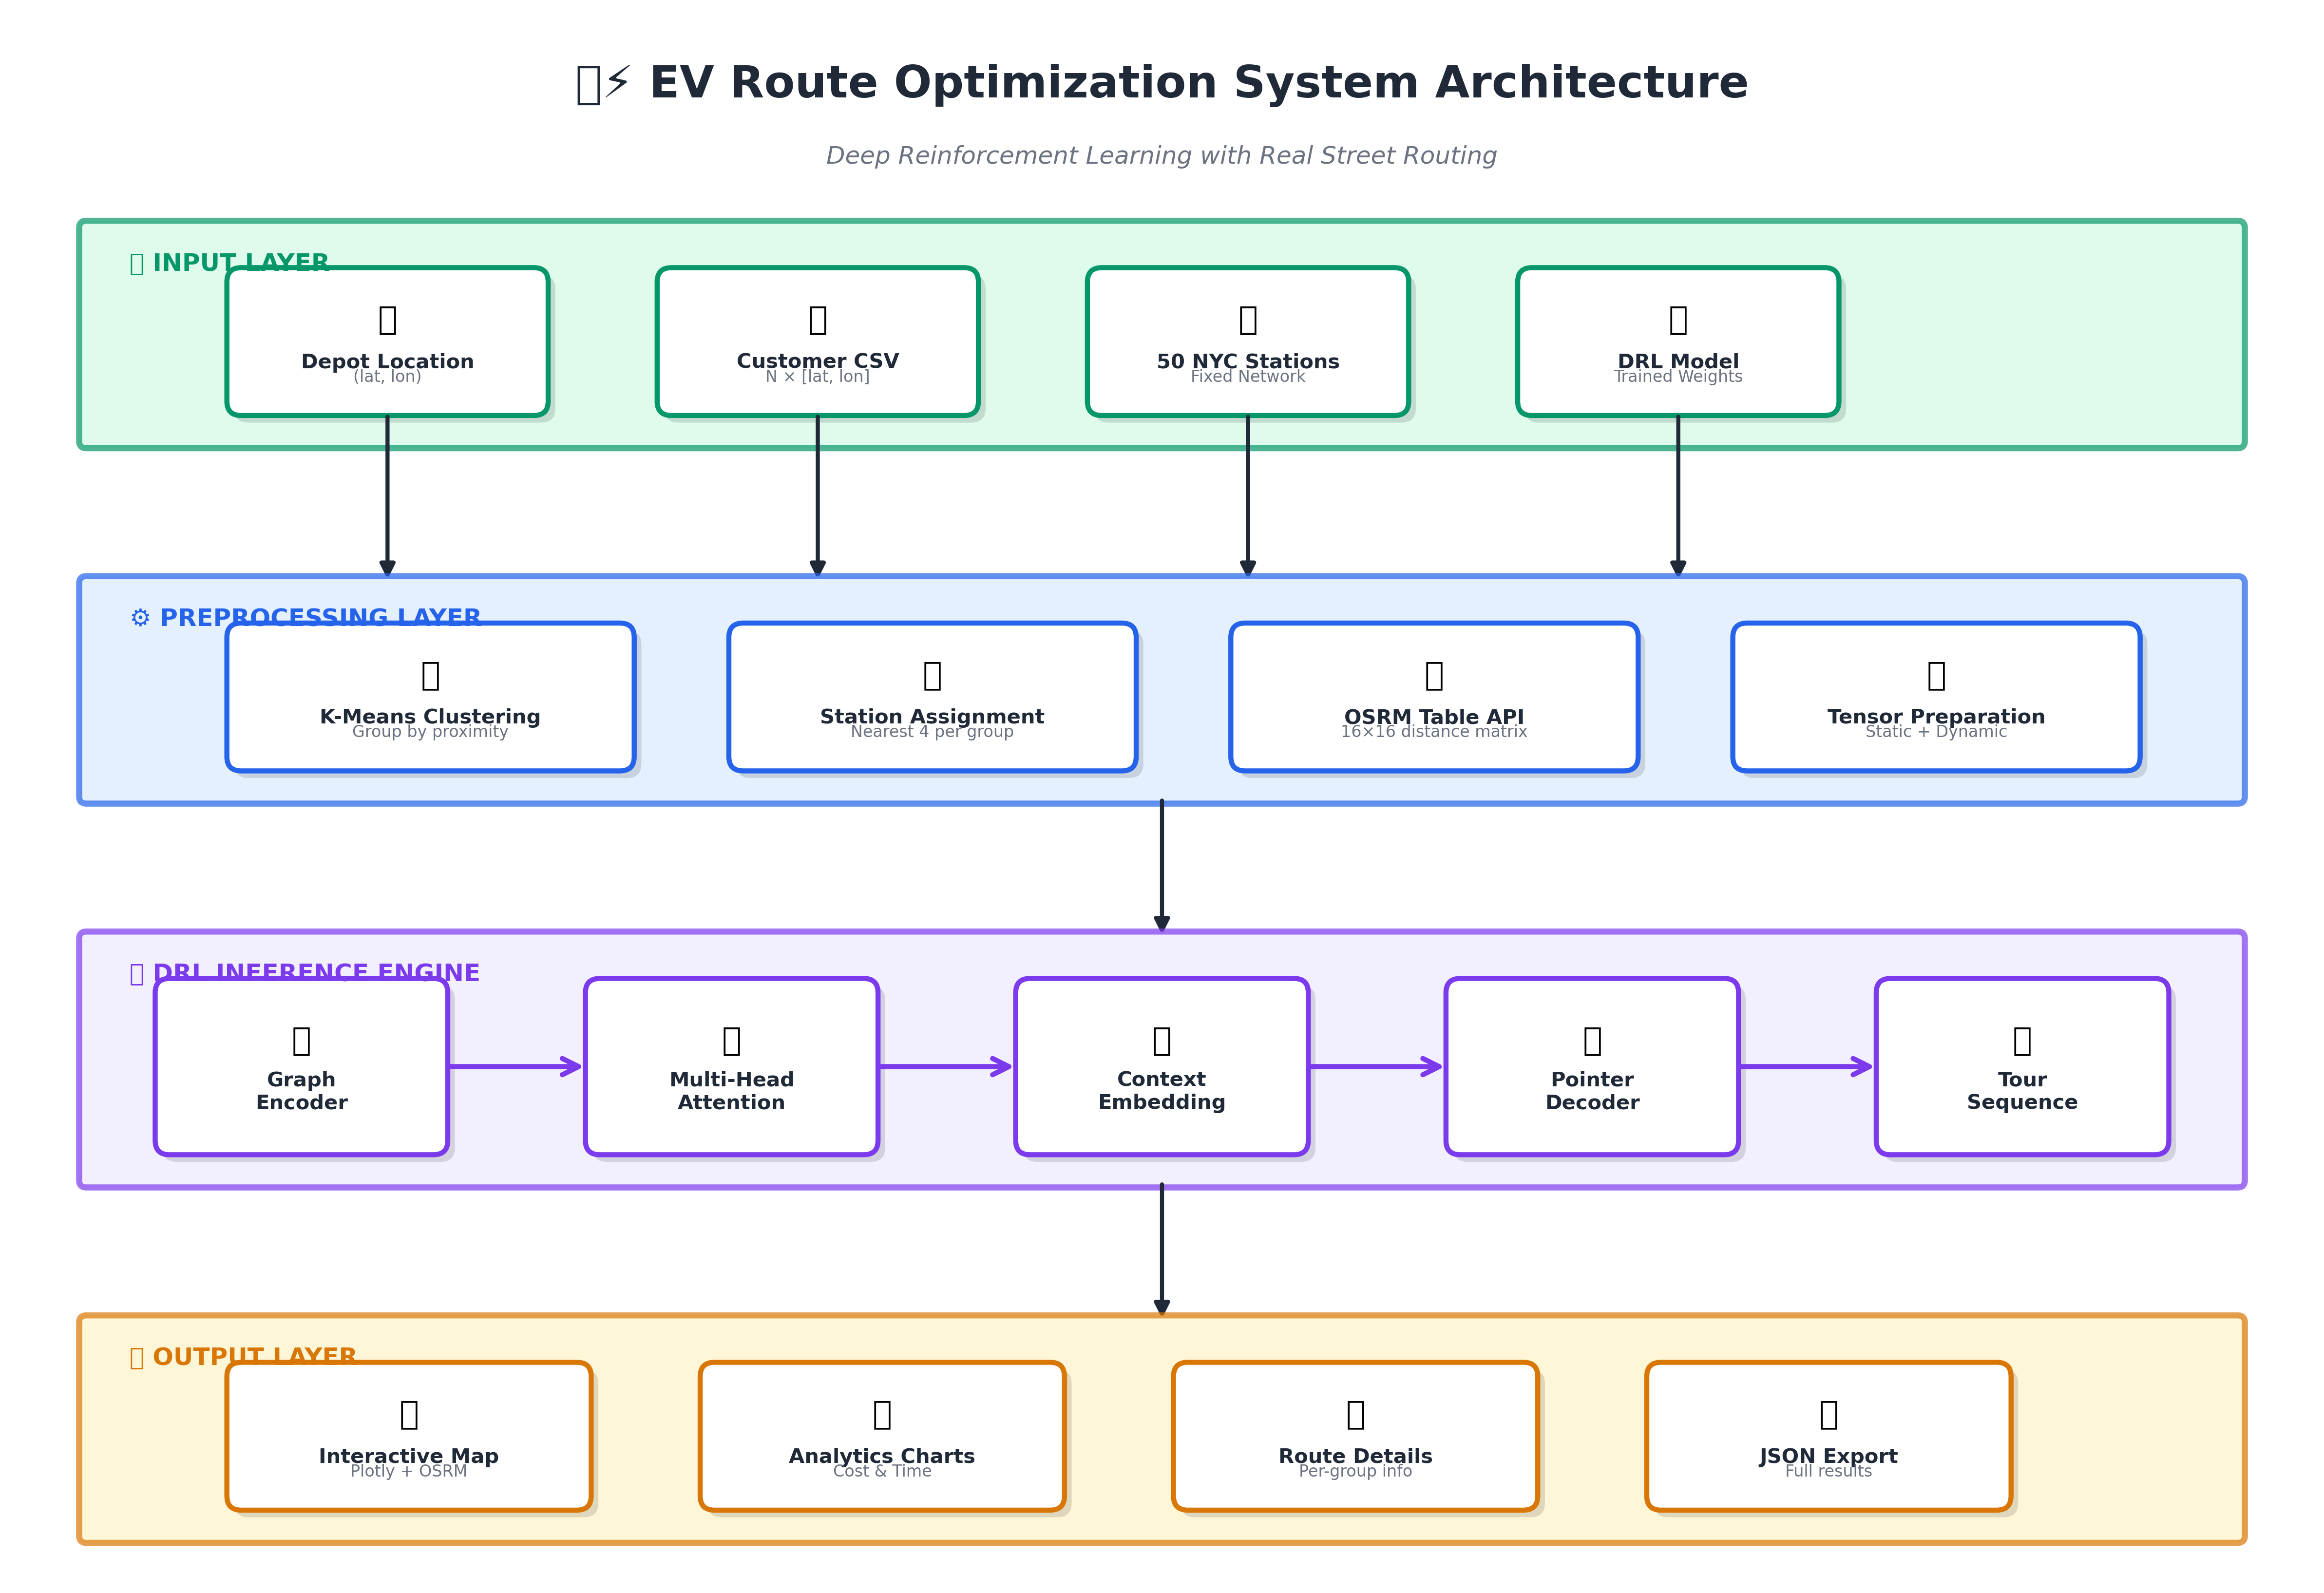
\includegraphics[width=0.72\textwidth]{system_architecture.png}
    \end{center}
\end{frame}

%-------------------------------------------------------------------------
\begin{frame}{Real-World Deployment: OSRM Integration}
    \begin{columns}[T]
        \begin{column}{0.48\textwidth}
            \textbf{Open Source Routing Machine:}
            \begin{itemize}
                \item Production-grade routing engine
                \item Real street-level distances
                \item OpenStreetMap data
            \end{itemize}

            \vspace{0.3cm}
            \textbf{Pipeline:}
            \begin{enumerate}
                \item Upload customer GPS coordinates
                \item Query OSRM for distance matrix
                \item Run DRL inference
                \item Visualize on real map
            \end{enumerate}
        \end{column}
        \begin{column}{0.48\textwidth}
            \begin{block}{Scalability: K-means Clustering}
                \begin{itemize}
                    \item Group customers into batches
                    \item 10 customers per cluster
                    \item Run DRL on each cluster
                    \item Combine results
                \end{itemize}
            \end{block}

            \begin{exampleblock}{NYC Setup}
                50 pre-configured charging stations across New York City
            \end{exampleblock}
        \end{column}
    \end{columns}
\end{frame}

%-------------------------------------------------------------------------
\begin{frame}{Interactive Dashboard}
    \begin{center}
        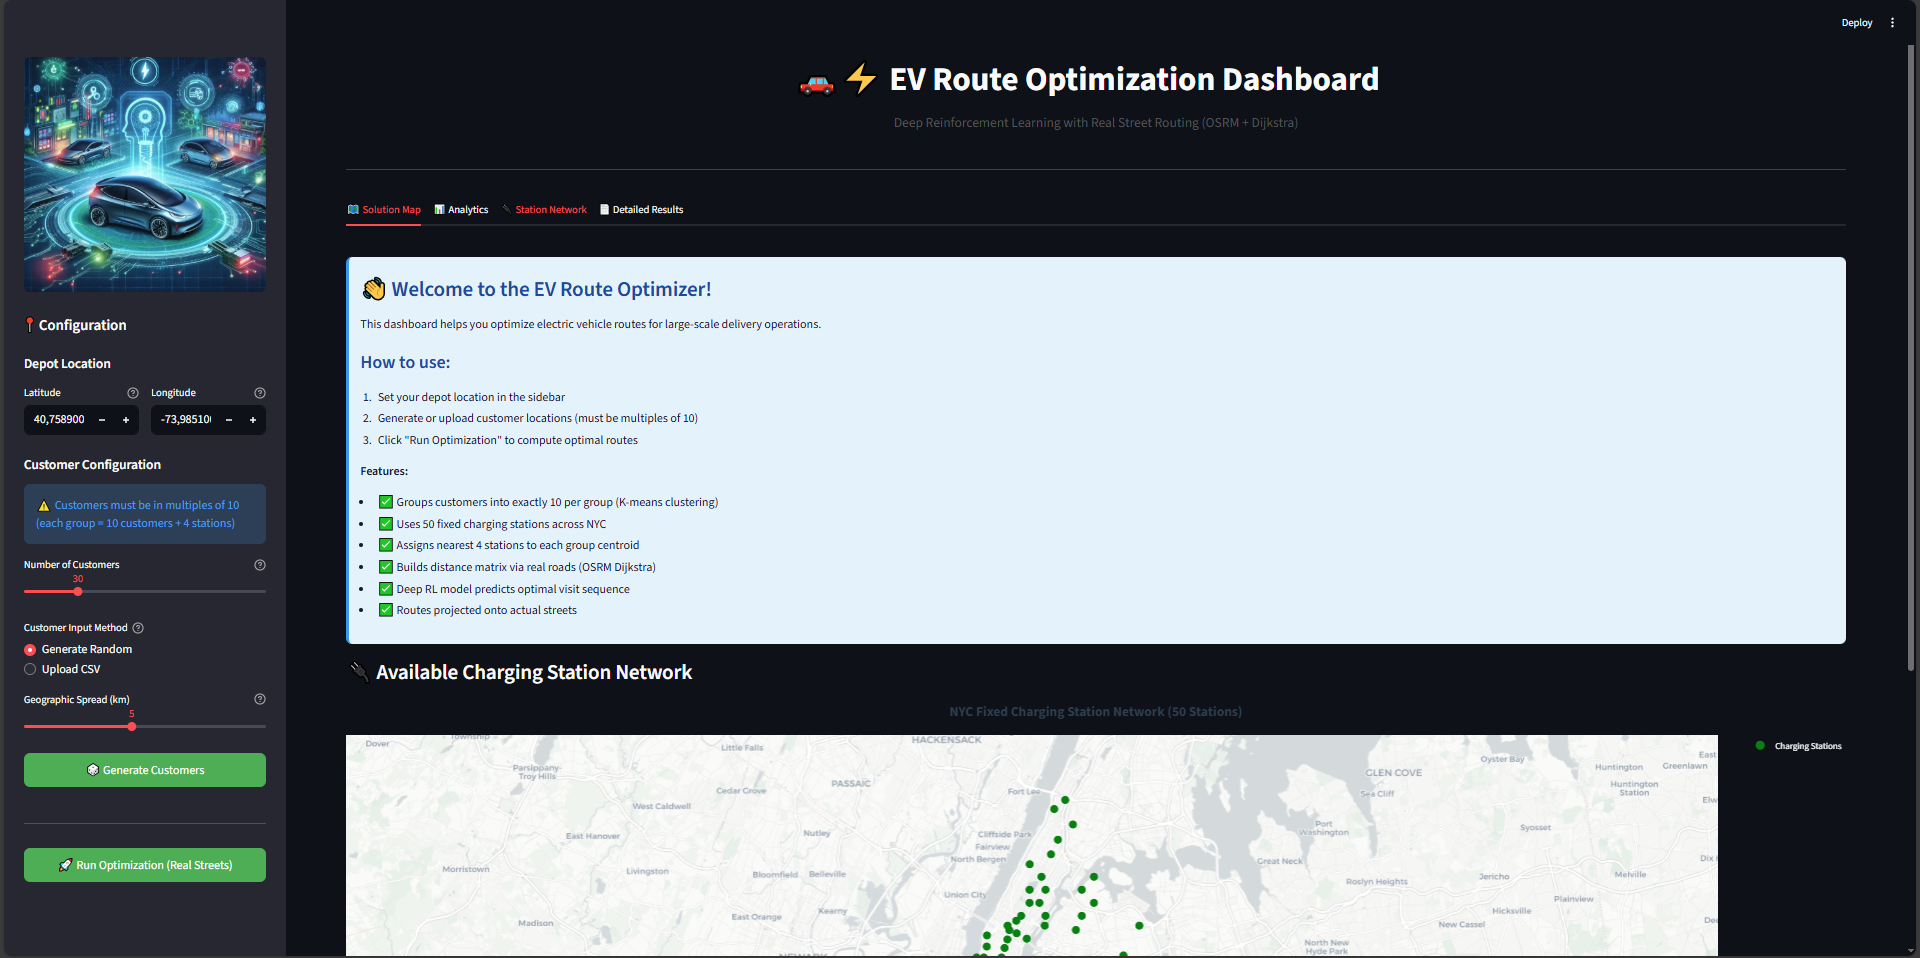
\includegraphics[width=0.78\textwidth]{main_page.PNG}
    \end{center}
    \small\centering Upload customers $\bullet$ Configure EV $\bullet$ Select stations $\bullet$ Real-time optimization
\end{frame}

%-------------------------------------------------------------------------
\begin{frame}{Route Optimization \& Results}
    \begin{columns}
        \begin{column}{0.48\textwidth}
            \begin{center}
                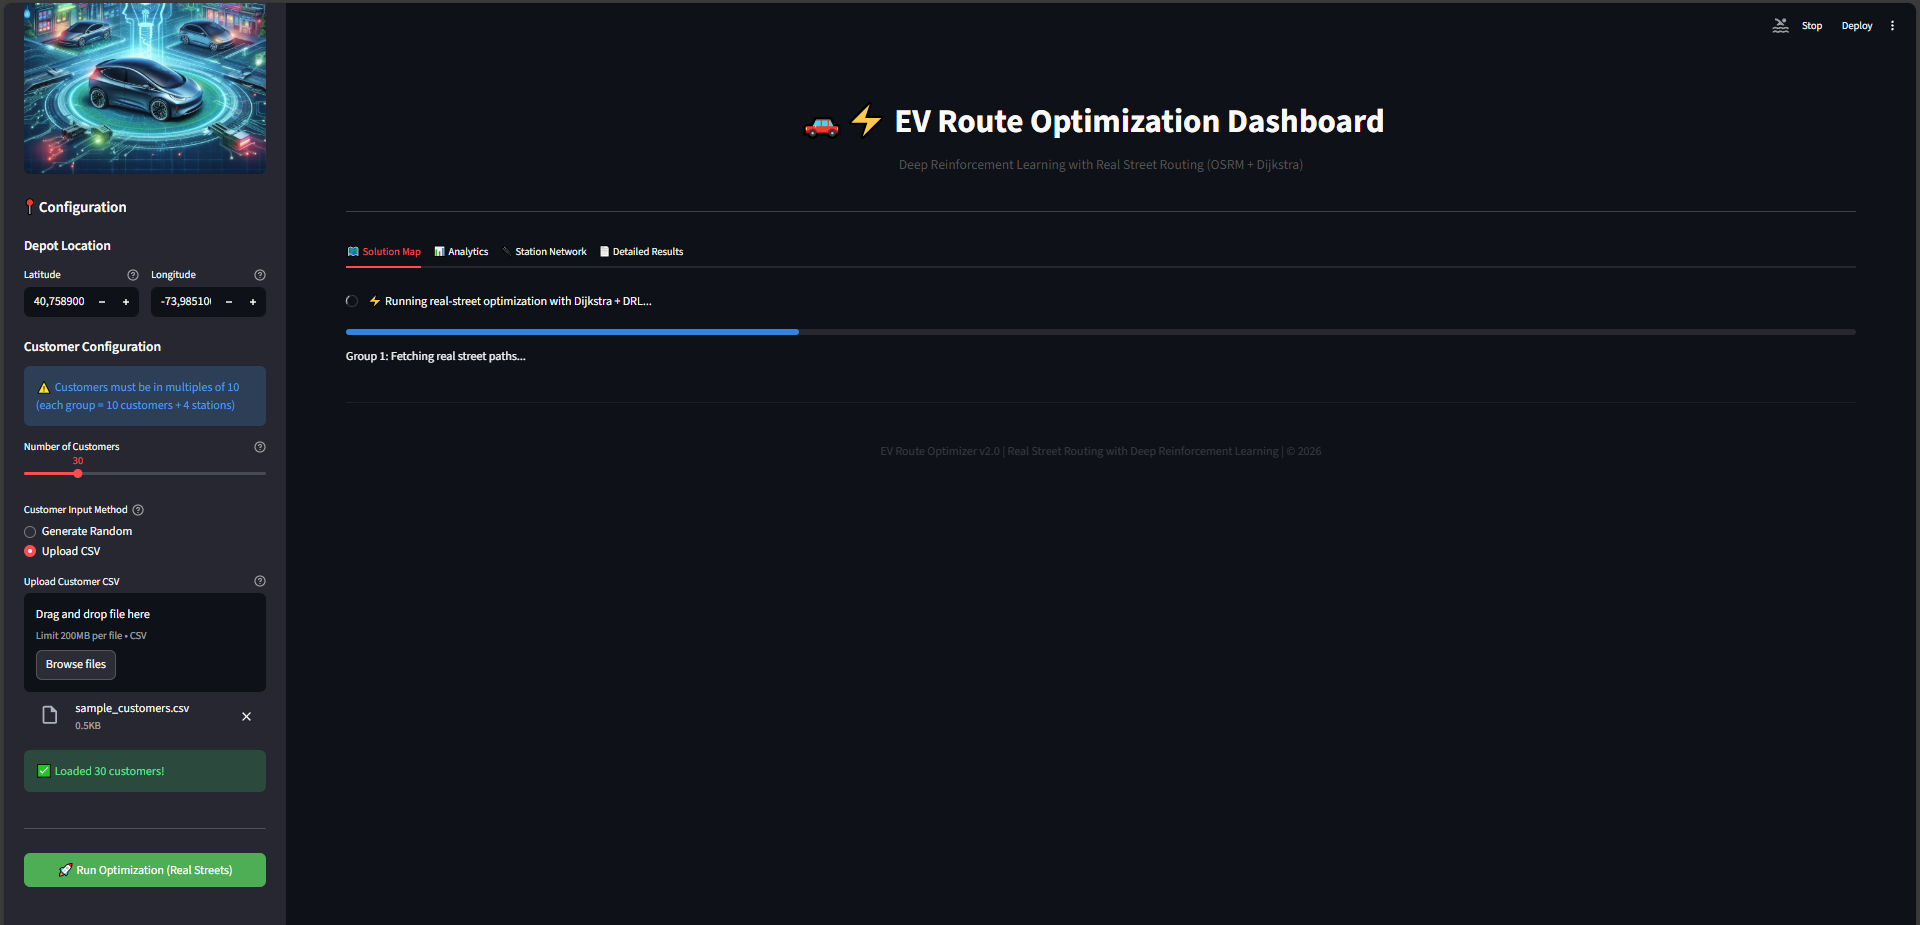
\includegraphics[width=\textwidth]{inference.PNG}
                \small\textbf{Inference Process}
            \end{center}
        \end{column}
        \begin{column}{0.48\textwidth}
            \begin{center}
                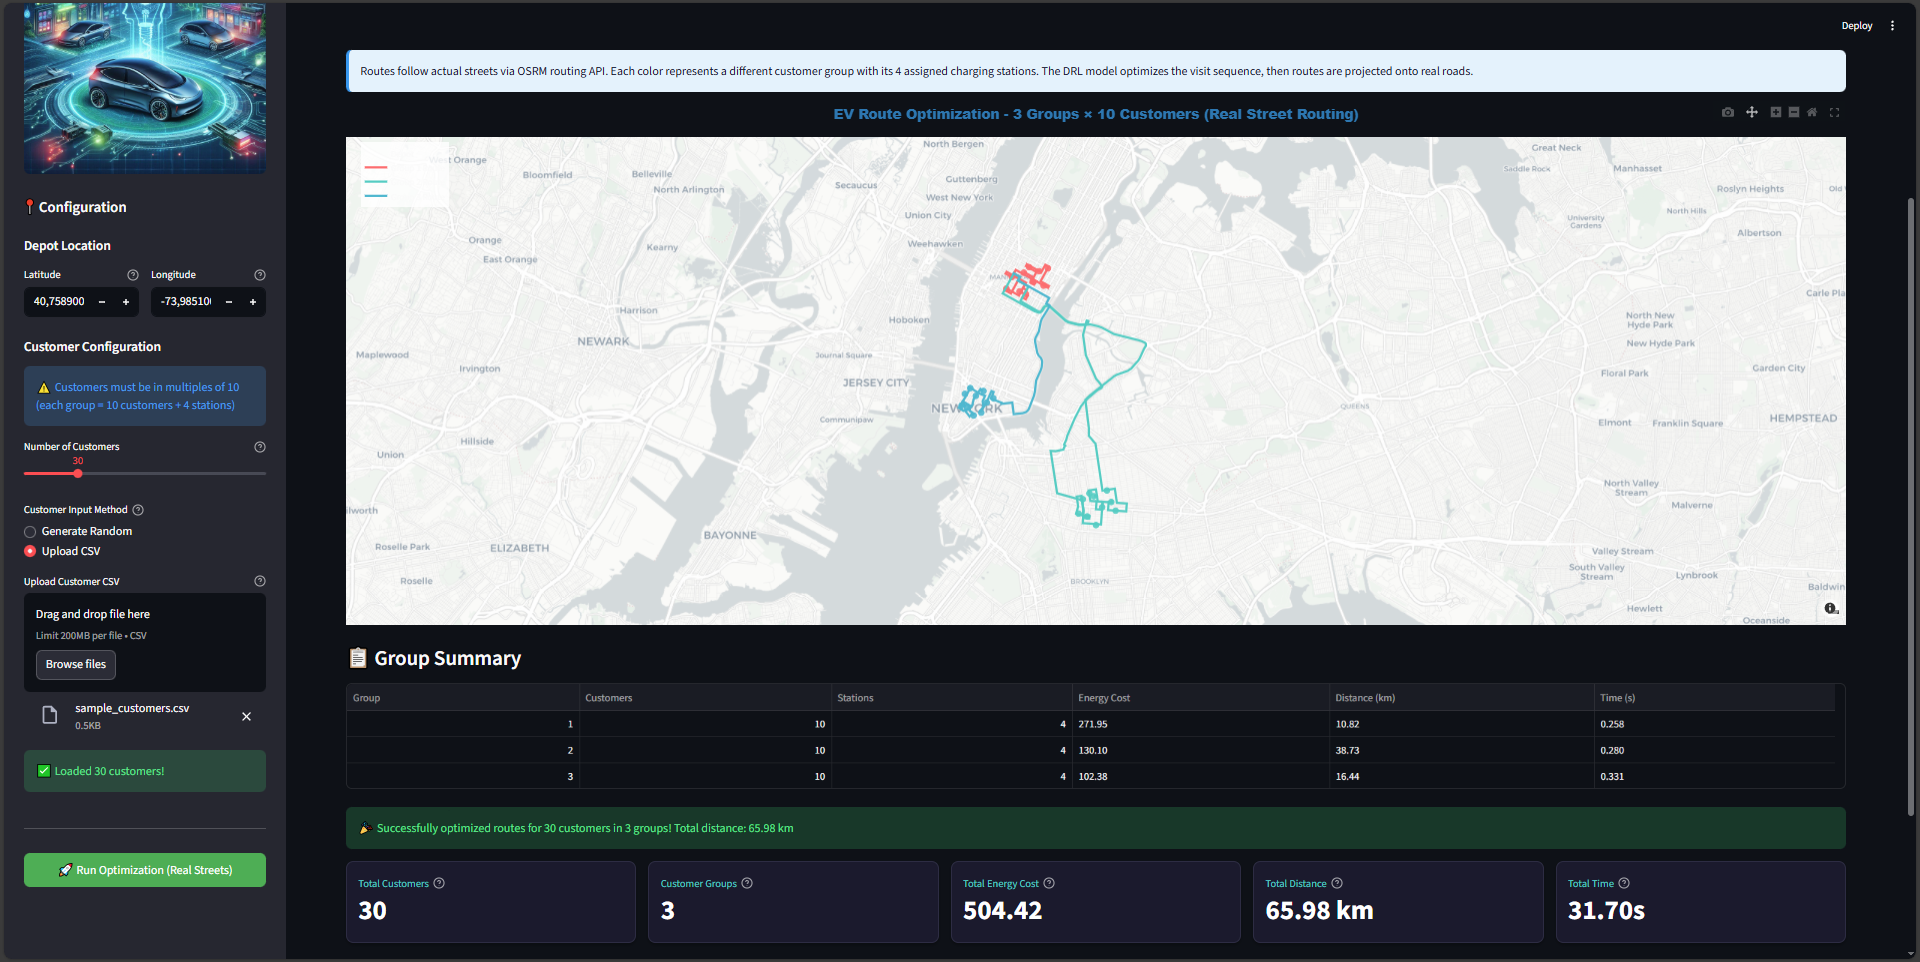
\includegraphics[width=\textwidth]{result.PNG}
                \small\textbf{Optimized Routes}
            \end{center}
        \end{column}
    \end{columns}
\end{frame}

%-------------------------------------------------------------------------
\begin{frame}{Analytics Dashboard}
    \begin{columns}
        \begin{column}{0.48\textwidth}
            \begin{center}
                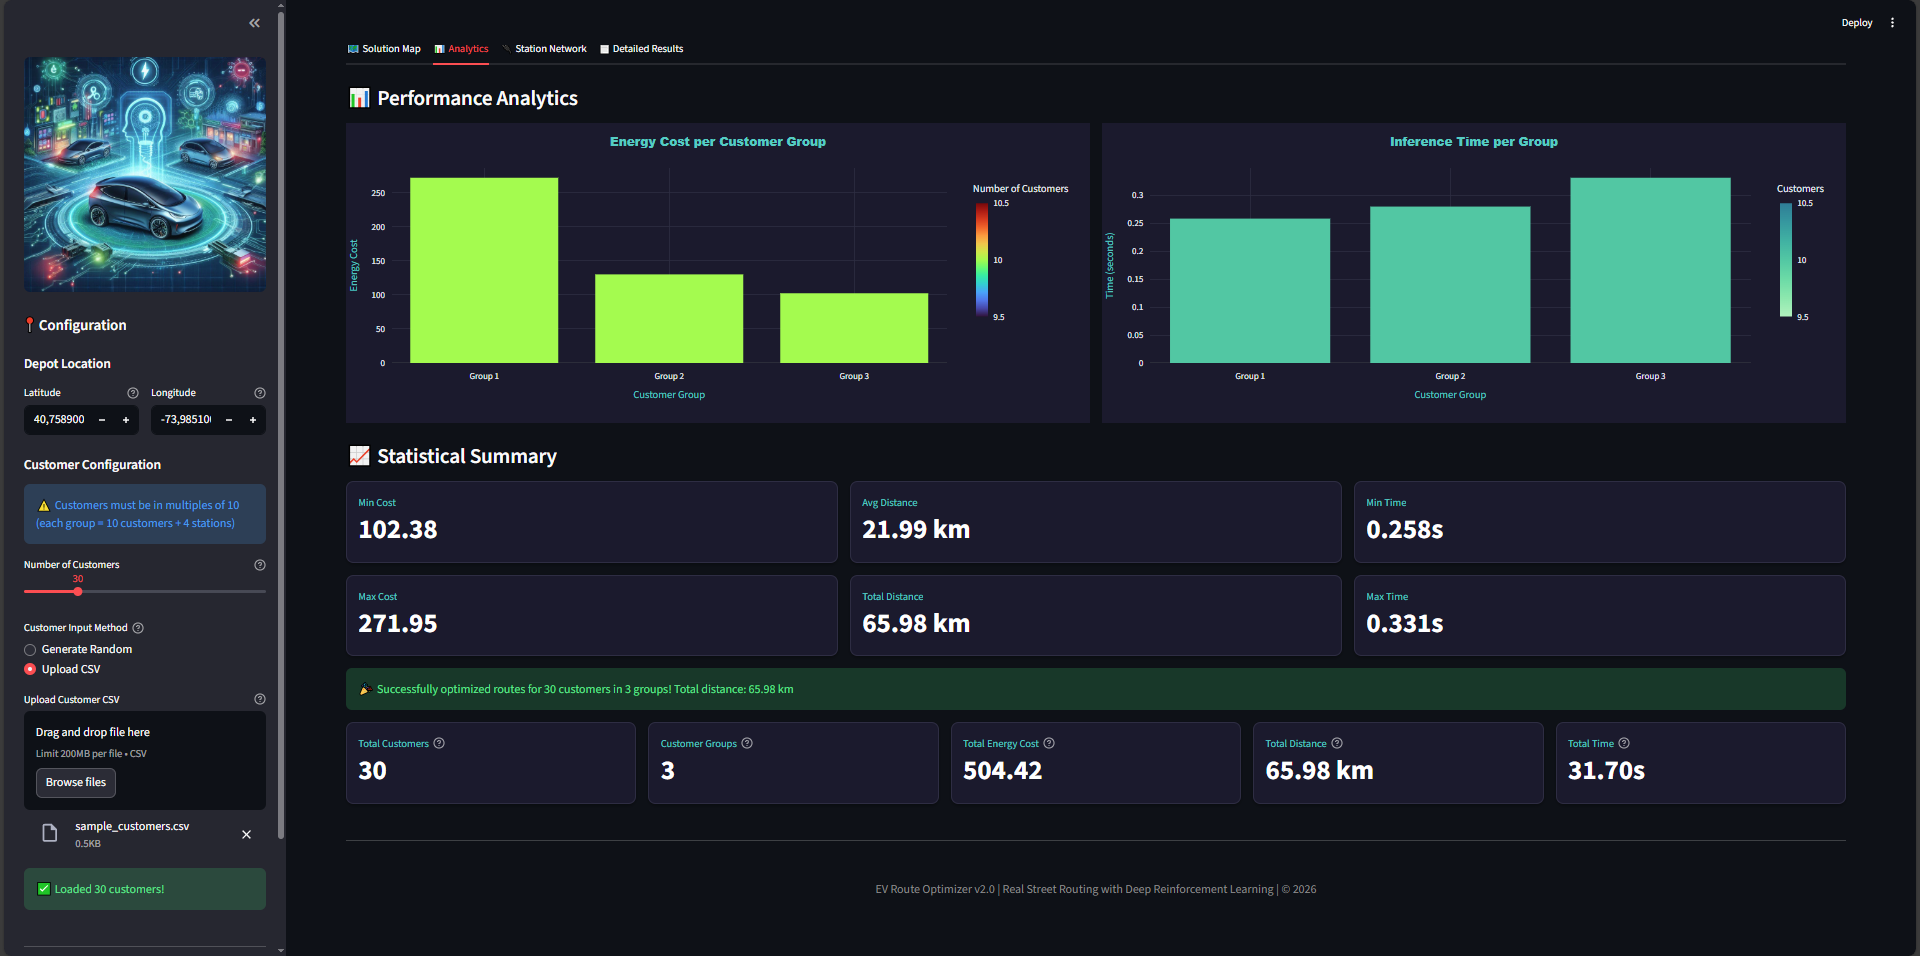
\includegraphics[width=\textwidth]{analytics.PNG}
            \end{center}
        \end{column}
        \begin{column}{0.48\textwidth}
            \begin{center}
                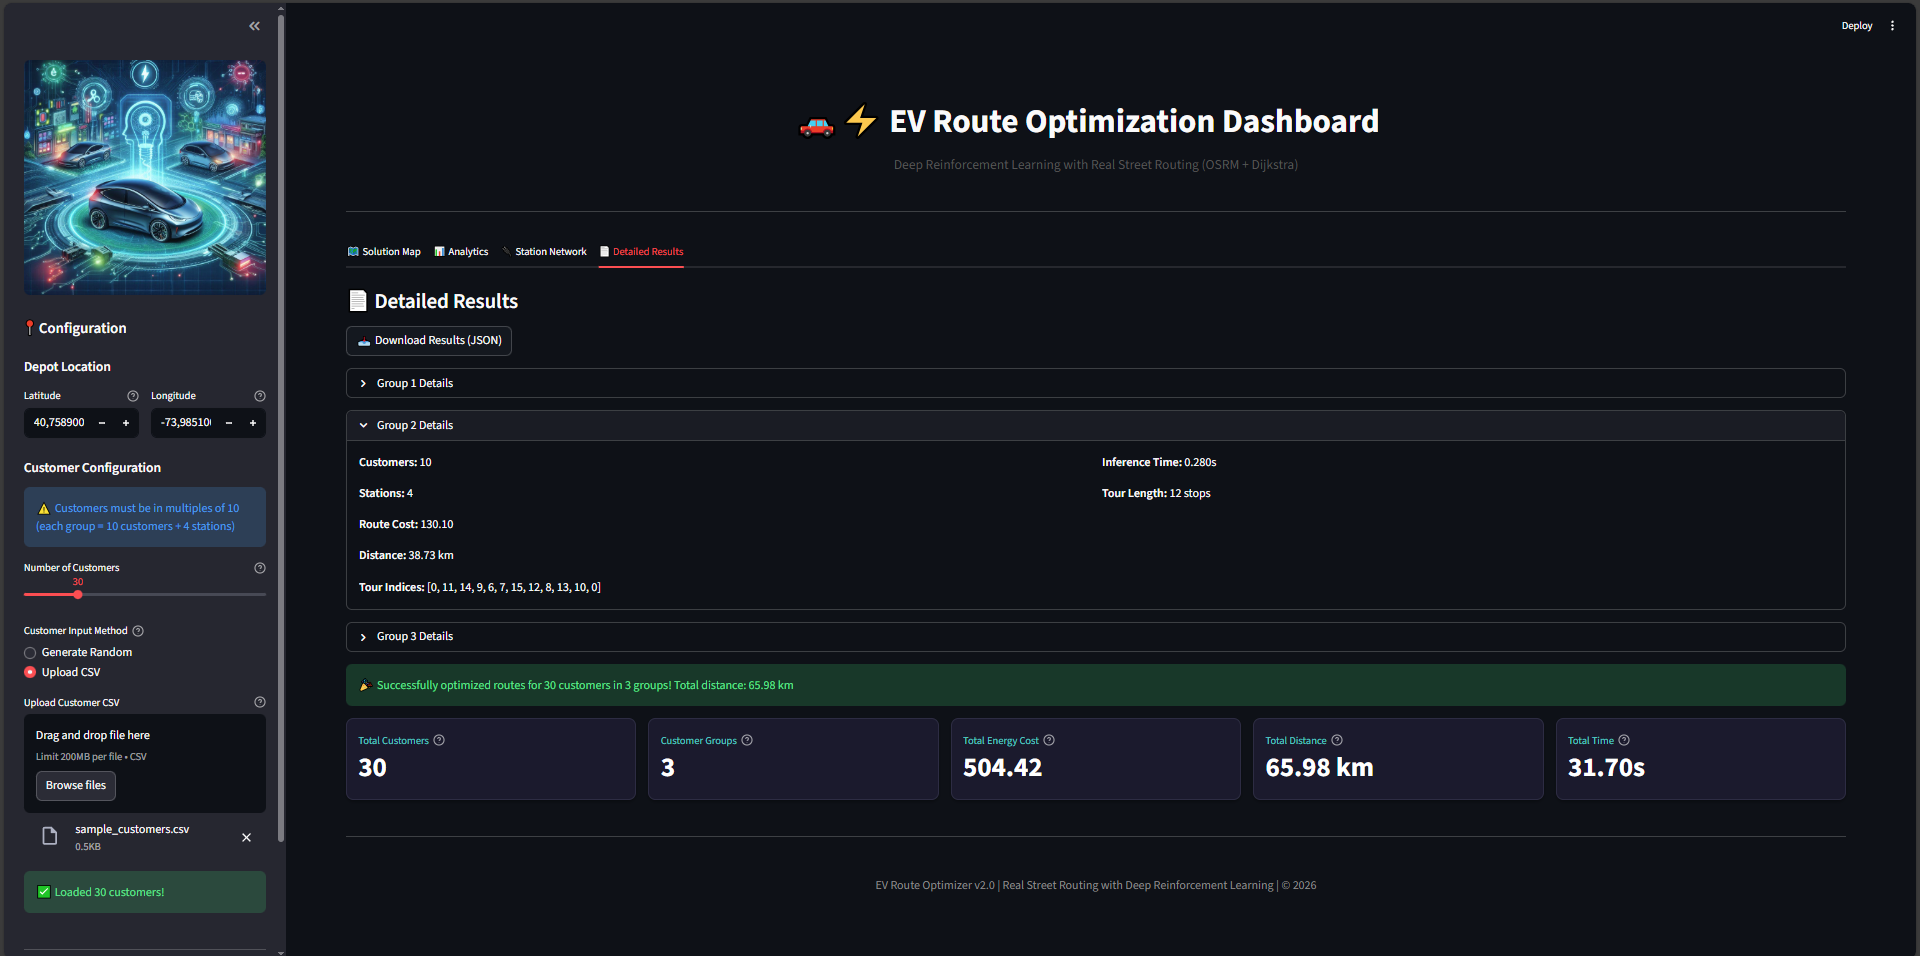
\includegraphics[width=\textwidth]{detailed.PNG}
            \end{center}
        \end{column}
    \end{columns}

    \vspace{0.3cm}
    \small Energy breakdown $\bullet$ SOC tracking $\bullet$ Cost analysis $\bullet$ JSON export
\end{frame}

%=========================================================================
\section{Optimization Methods}
%=========================================================================

%-------------------------------------------------------------------------
\begin{frame}{Baseline Methods Overview}
    \begin{columns}[T]
        \begin{column}{0.48\textwidth}
            \begin{block}{OR-Tools (Google)}
                Constraint programming + local search
            \end{block}

            \begin{block}{Hill Climbing}
                Local search: 2-opt, Or-opt, Exchange\\
                Fast but trapped in local optima
            \end{block}
        \end{column}
        \begin{column}{0.48\textwidth}
            \begin{block}{Simulated Annealing}
                $P(\text{accept}) = e^{-\Delta E/T}$\\
                Escapes local optima via temperature
            \end{block}

            \begin{block}{Ant Colony Optimization}
                Pheromone-based collective search\\
                Good for combinatorial problems
            \end{block}
        \end{column}
    \end{columns}

    \vspace{0.4cm}
    \begin{center}
        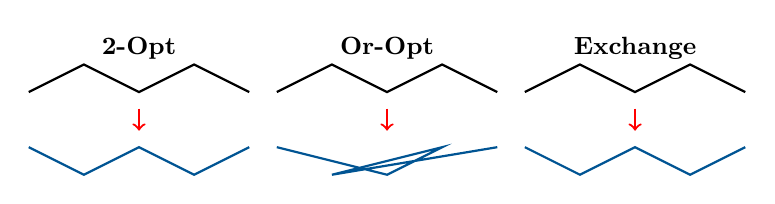
\begin{tikzpicture}[scale=0.7]
            % 2-opt
            \node[font=\bfseries\small] at (-4.5, 1.8) {2-Opt};
            \draw[thick] (-6.5,1) -- (-5.5,1.5) -- (-4.5,1) -- (-3.5,1.5) -- (-2.5,1);
            \draw[thick, primaryblue] (-6.5,0) -- (-5.5,-0.5) -- (-4.5,0) -- (-3.5,-0.5) -- (-2.5,0);
            \draw[->, thick, red] (-4.5, 0.7) -- (-4.5, 0.3);

            % Or-opt
            \node[font=\bfseries\small] at (0, 1.8) {Or-Opt};
            \draw[thick] (-2,1) -- (-1,1.5) -- (0,1) -- (1,1.5) -- (2,1);
            \draw[thick, primaryblue] (-2,0) -- (0,-0.5) -- (1,0) -- (-1,-0.5) -- (2,0);
            \draw[->, thick, red] (0, 0.7) -- (0, 0.3);

            % Exchange
            \node[font=\bfseries\small] at (4.5, 1.8) {Exchange};
            \draw[thick] (2.5,1) -- (3.5,1.5) -- (4.5,1) -- (5.5,1.5) -- (6.5,1);
            \draw[thick, primaryblue] (2.5,0) -- (3.5,-0.5) -- (4.5,0) -- (5.5,-0.5) -- (6.5,0);
            \draw[->, thick, red] (4.5, 0.7) -- (4.5, 0.3);
        \end{tikzpicture}
    \end{center}
\end{frame}

%-------------------------------------------------------------------------
\begin{frame}{Simulated Annealing: Convergence Behavior}
    \begin{columns}[T]
        \begin{column}{0.55\textwidth}
            \begin{center}
                % SA Convergence Plot
                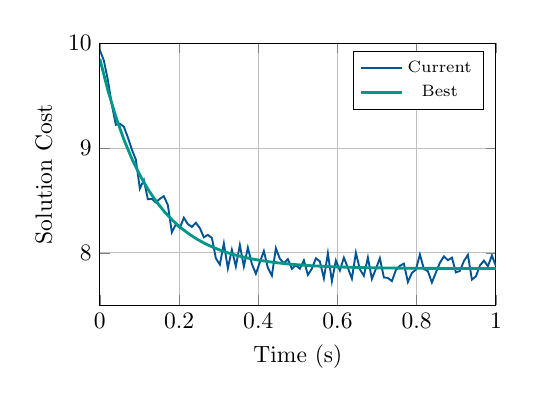
\begin{tikzpicture}[scale=0.85]
                    \begin{axis}[
                        width=7.5cm, height=5.5cm,
                        xlabel={Time (s)},
                        ylabel={Solution Cost},
                        xmin=0, xmax=1,
                        ymin=7.5, ymax=10,
                        grid=major,
                        legend pos=north east,
                        legend style={font=\scriptsize}
                    ]
                    % Simulated SA convergence curve
                    \addplot[primaryblue, thick, domain=0:1, samples=100]
                        {7.85 + 2*exp(-8*x) + 0.15*rand};
                    \addlegendentry{Current}
                    \addplot[accentgreen, very thick, domain=0:1, samples=50]
                        {7.85 + 2*exp(-8*x)};
                    \addlegendentry{Best}
                    \end{axis}
                \end{tikzpicture}
            \end{center}
        \end{column}
        \begin{column}{0.42\textwidth}
            \begin{block}{Key Observations}
                \begin{itemize}
                    \item High variance early (exploration)
                    \item Gradual convergence
                    \item Track \textbf{best-ever} solution
                    \item Plateau before time limit
                \end{itemize}
            \end{block}

            \begin{alertblock}{Parameter Sensitivity}
                $T_{\text{start}}$ and $T_{\text{end}}$ critically affect solution quality
            \end{alertblock}
        \end{column}
    \end{columns}
\end{frame}

%=========================================================================
\section{Deep Reinforcement Learning}
%=========================================================================

%-------------------------------------------------------------------------
\begin{frame}{Why Deep Reinforcement Learning?}
    \begin{columns}[T]
        \begin{column}{0.48\textwidth}
            \begin{alertblock}{Traditional Limitations}
                \begin{itemize}
                    \item Exact: exponential time
                    \item Heuristics: problem-specific
                    \item No generalization
                    \item Slow for real-time
                \end{itemize}
            \end{alertblock}
        \end{column}
        \begin{column}{0.48\textwidth}
            \begin{exampleblock}{DRL Advantages}
                \begin{itemize}
                    \item \textbf{Learn} to solve
                    \item \textbf{Generalize} to new instances
                    \item \textbf{Fast inference} (ms)
                    \item \textbf{End-to-end} optimization
                \end{itemize}
            \end{exampleblock}
        \end{column}
    \end{columns}

    \vspace{0.5cm}
    \begin{block}{Key Idea}
        \centering
        Train a neural network to \textbf{construct} solutions step-by-step,\\
        learning which decisions minimize energy consumption
    \end{block}

    \vspace{0.2cm}
    \centering\small Based on: Kool et al., ``Attention, Learn to Solve Routing Problems!'' (ICLR 2019)
\end{frame}

%-------------------------------------------------------------------------
\begin{frame}{Attention-Based Architecture}
    \begin{center}
        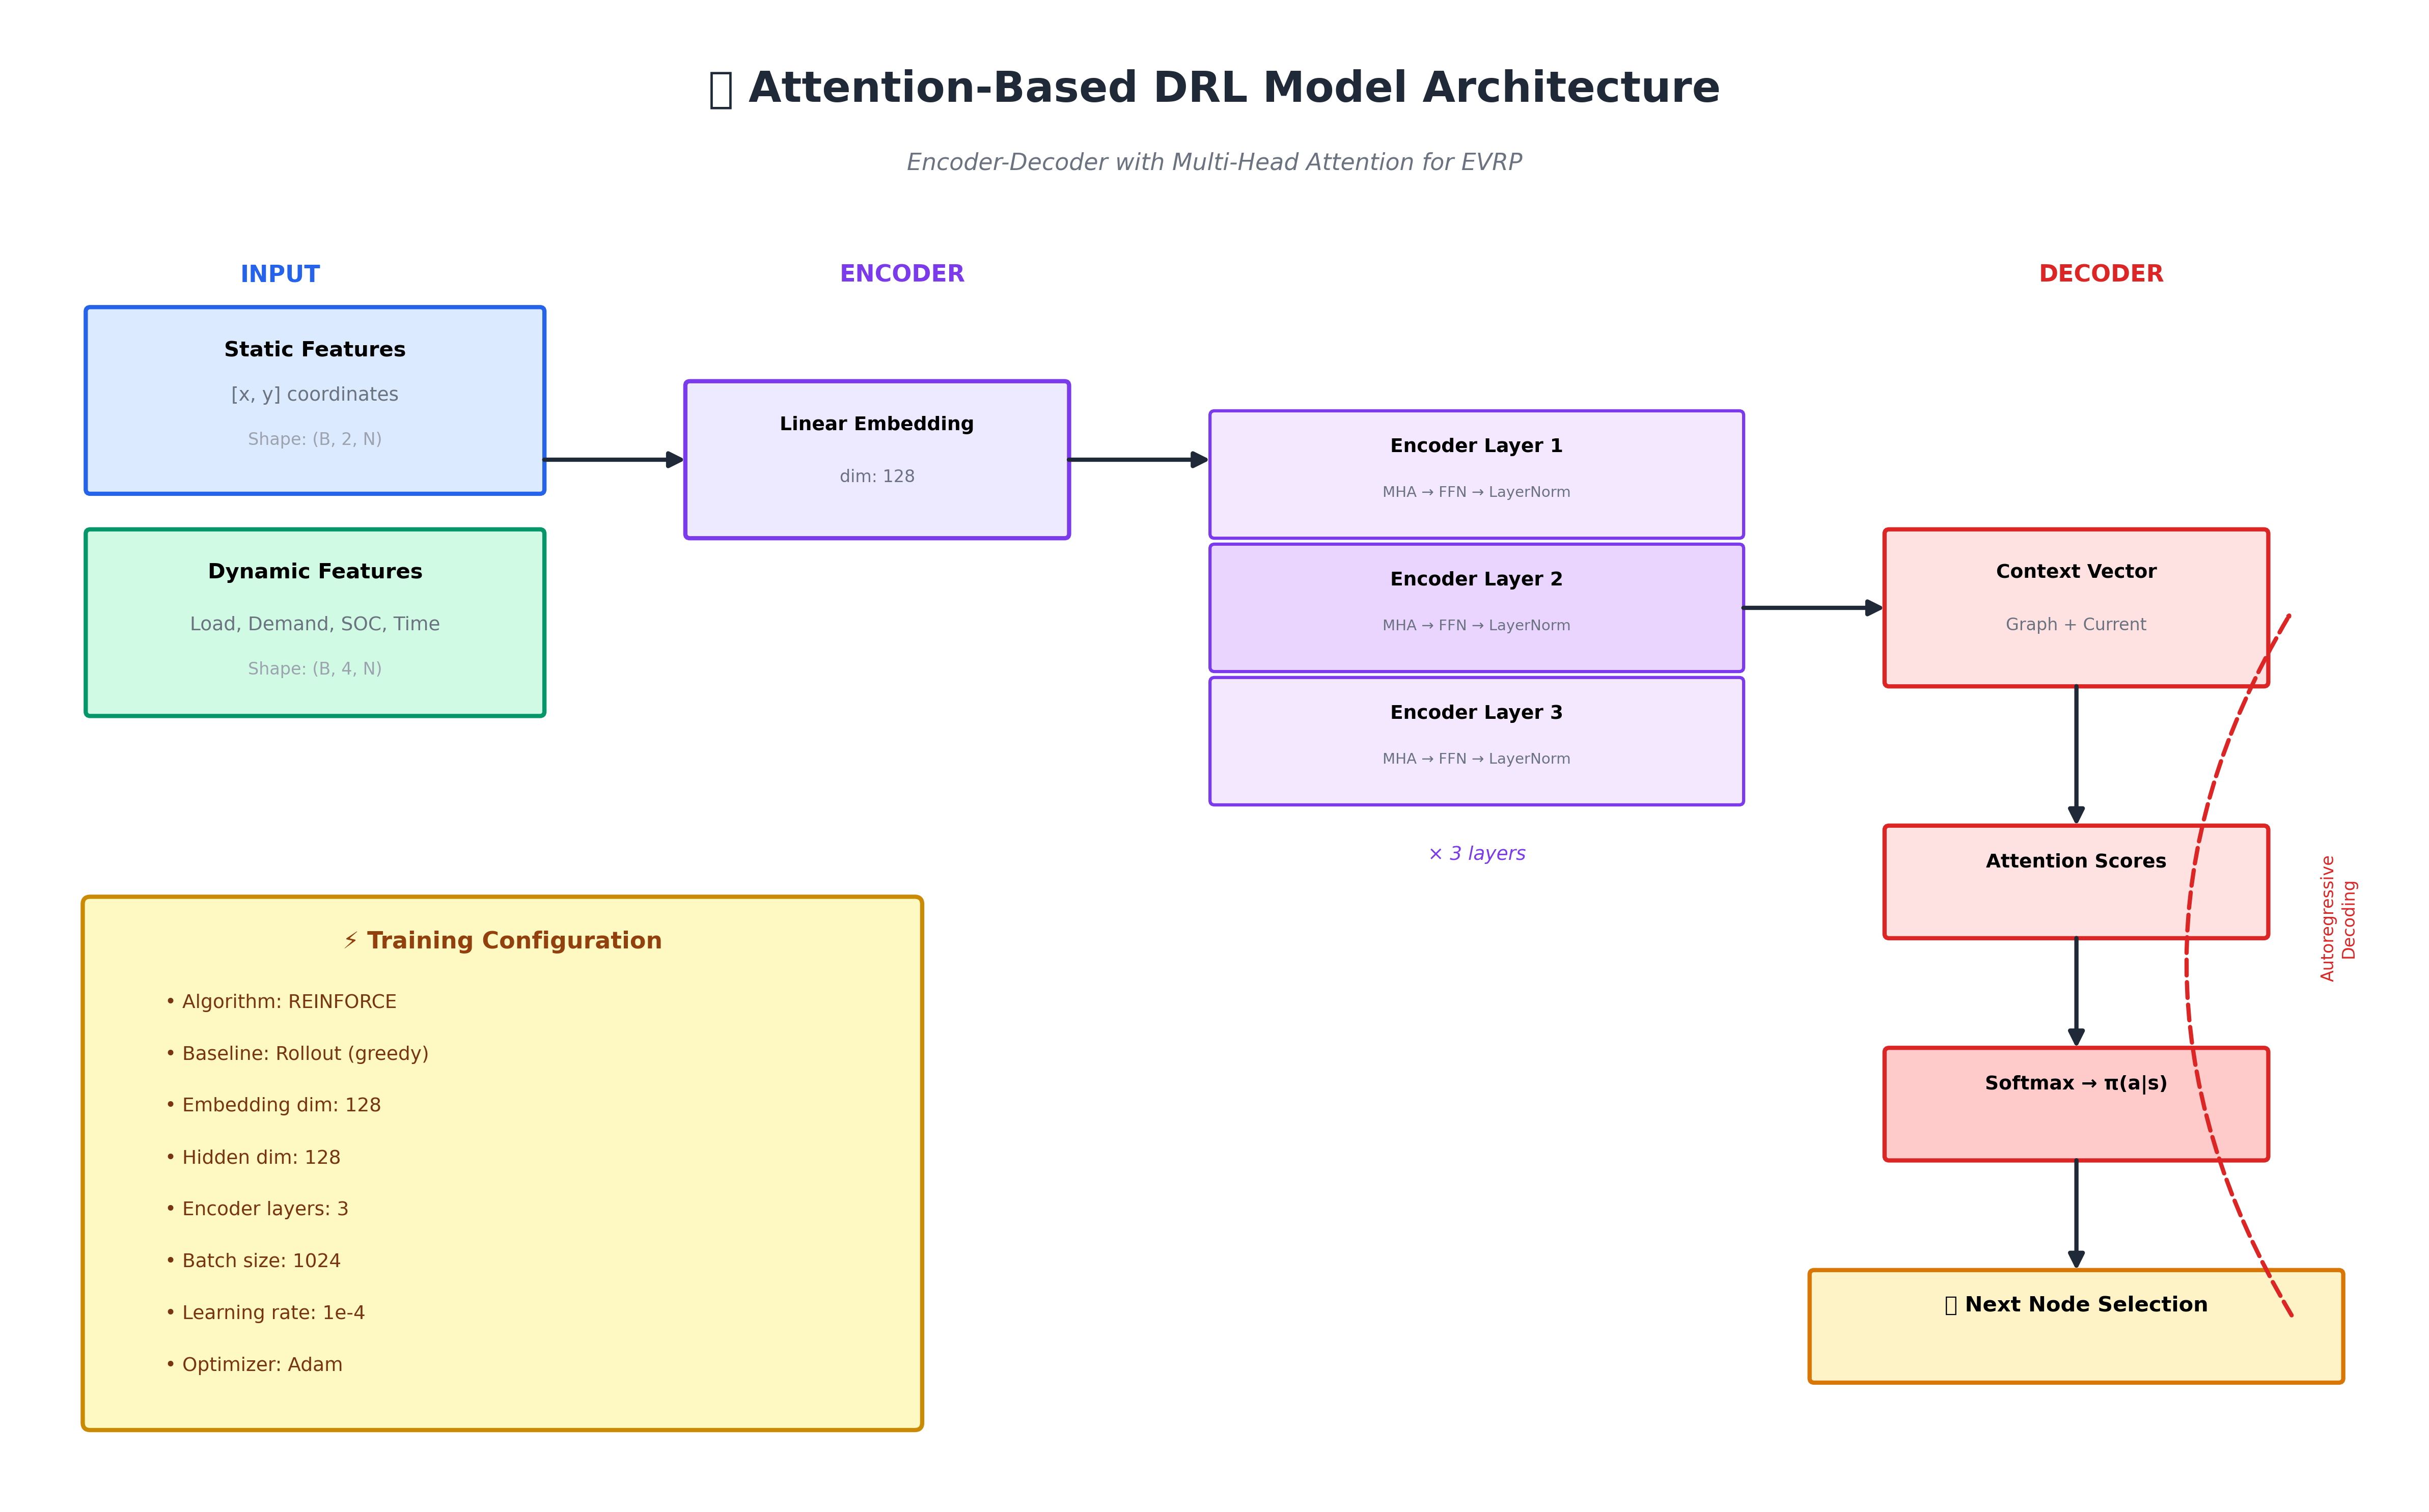
\includegraphics[width=0.58\textwidth]{drl_model_architecture.png}
    \end{center}

    \begin{columns}[T]
        \begin{column}{0.48\textwidth}
            \begin{block}{Encoder}
                Multi-head self-attention\\
                Captures node relationships
            \end{block}
        \end{column}
        \begin{column}{0.48\textwidth}
            \begin{block}{Decoder}
                Autoregressive generation\\
                Masked attention for feasibility
            \end{block}
        \end{column}
    \end{columns}
\end{frame}

%-------------------------------------------------------------------------
\begin{frame}{MDP Formulation \& Training}
    \begin{columns}[T]
        \begin{column}{0.48\textwidth}
            \begin{block}{MDP Components}
                \begin{description}
                    \item[State] Partial solution + vehicle status
                    \item[Action] Select next node
                    \item[Reward] Negative energy consumed
                    \item[Policy] Neural network $\pi_\theta$
                \end{description}
            \end{block}
        \end{column}
        \begin{column}{0.48\textwidth}
            \begin{block}{REINFORCE with Baseline}
                \[
                \nabla J \approx \frac{1}{B}\sum_{i} (L_i - b_i) \nabla \log p_\theta
                \]
                \small Rollout baseline reduces variance
            \end{block}
        \end{column}
    \end{columns}

    \vspace{0.4cm}
    \begin{block}{EV-Specific Features}
        \begin{itemize}
            \item SOC tracking: $\text{SOC}_{t+1} = \text{SOC}_t - E_{ij}/E_{\text{battery}}$
            \item Load dynamics: cargo decreases after delivery
            \item Dynamic masking: feasibility constraints enforced
        \end{itemize}
    \end{block}
\end{frame}

%=========================================================================
\section{Results}
%=========================================================================

%-------------------------------------------------------------------------
\begin{frame}{Training Results}
    \begin{center}
        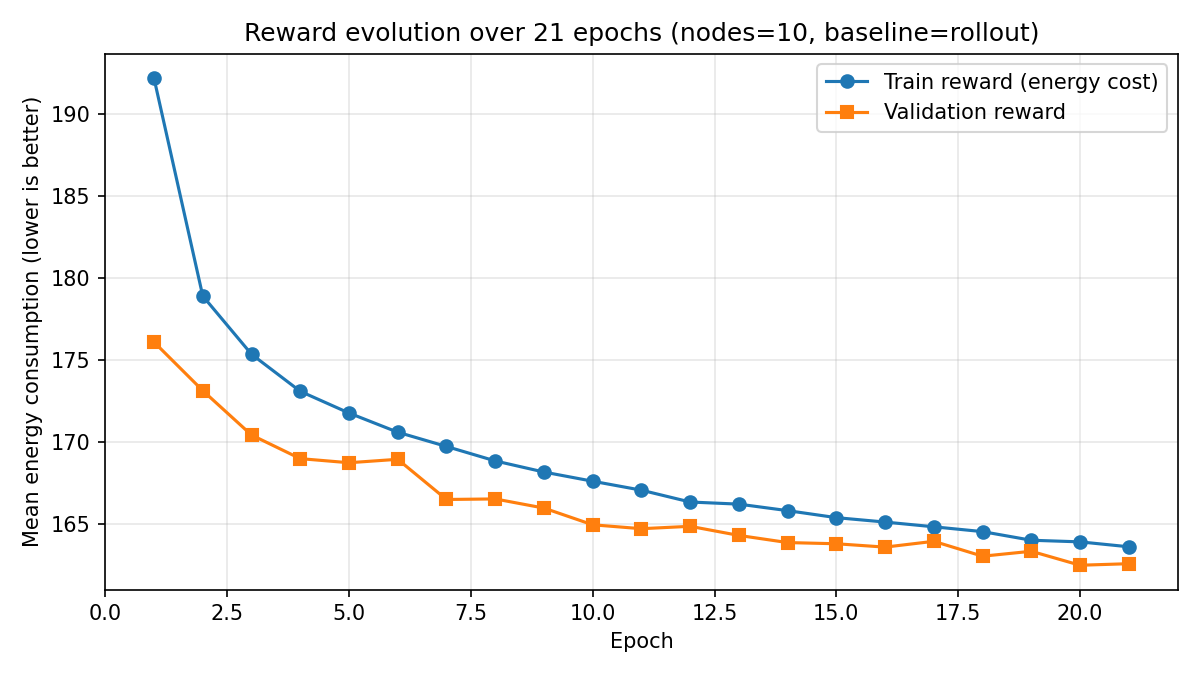
\includegraphics[width=0.6\textwidth]{training_reward.png}
    \end{center}

    \begin{columns}[T]
        \begin{column}{0.48\textwidth}
            \begin{block}{Configuration}
                \small 10 customers, 4 stations, 20 epochs, batch 1024
            \end{block}
        \end{column}
        \begin{column}{0.48\textwidth}
            \begin{block}{Observation}
                \small Consistent improvement, no overfitting
            \end{block}
        \end{column}
    \end{columns}
\end{frame}

%-------------------------------------------------------------------------
\begin{frame}{Performance Comparison}
    \begin{center}
        \begin{tabular}{lcc}
            \toprule
            \textbf{Method} & \textbf{Energy (kWh)} & \textbf{Time} \\
            \midrule
            \textbf{OR-Tools} & \textbf{11.92} & 2.1s \\
            \rowcolor{lightgray} DRL (Ours) & 12.18 & \textbf{0.5s} \\
            Ant Colony & 12.67 & 3.2s \\
            Simulated Annealing & 12.89 & 1.5s \\
            Hill Climbing & 13.21 & 0.8s \\
            \bottomrule
        \end{tabular}
    \end{center}

    \vspace{0.5cm}
    \begin{columns}[T]
        \begin{column}{0.48\textwidth}
            \begin{exampleblock}{Solution Quality}
                \begin{itemize}
                    \item Only \textbf{2.2\%} gap vs OR-Tools
                    \item \textbf{7.8\%} better than Hill Climbing
                \end{itemize}
            \end{exampleblock}
        \end{column}
        \begin{column}{0.48\textwidth}
            \begin{exampleblock}{Speed}
                \begin{itemize}
                    \item \textbf{4x} faster than OR-Tools
                    \item \textbf{6x} faster than ACO
                \end{itemize}
            \end{exampleblock}
        \end{column}
    \end{columns}
\end{frame}

%=========================================================================
\section{Conclusion}
%=========================================================================

%-------------------------------------------------------------------------
\begin{frame}{Summary \& Contributions}
    \begin{columns}[T]
        \begin{column}{0.48\textwidth}
            \begin{block}{What We Built}
                \begin{enumerate}
                    \item Physics-based energy model
                    \item Baseline benchmarks (OR-Tools, SA, ACO, HC)
                    \item Attention-based DRL solver
                    \item Production-ready dashboard
                \end{enumerate}
            \end{block}
        \end{column}
        \begin{column}{0.48\textwidth}
            \begin{block}{Key Results}
                \begin{itemize}
                    \item \cmark~Near-optimal solutions
                    \item \cmark~4x faster inference
                    \item \cmark~Generalizes to new instances
                    \item \cmark~Real-world deployment ready
                \end{itemize}
            \end{block}
        \end{column}
    \end{columns}

    \vspace{0.4cm}
    \begin{exampleblock}{Future Work}
        \centering
        Scale to 50+ customers $\bullet$ Multi-depot $\bullet$ Dynamic traffic $\bullet$ Fleet coordination
    \end{exampleblock}
\end{frame}

%-------------------------------------------------------------------------
\begin{frame}[plain]
    \begin{center}
        \vspace{2cm}
        {\Huge\textbf{Thank You!}}

        \vspace{1cm}
        {\large Questions?}
    \end{center}
\end{frame}

%-------------------------------------------------------------------------
\begin{frame}{References}
    \small
    \begin{thebibliography}{99}
        \bibitem{kool} W. Kool et al., \textit{``Attention, Learn to Solve Routing Problems!''}, ICLR 2019.
        \bibitem{kirkpatrick} S. Kirkpatrick et al., \textit{``Optimization by Simulated Annealing''}, Science 1983.
        \bibitem{dorigo} M. Dorigo et al., \textit{``The Ant System''}, IEEE Trans. SMC 1996.
        \bibitem{vaswani} A. Vaswani et al., \textit{``Attention Is All You Need''}, NeurIPS 2017.
        \bibitem{ortools} Google OR-Tools. \url{https://developers.google.com/optimization}
        \bibitem{osrm} Project OSRM. \url{http://project-osrm.org/}
    \end{thebibliography}
\end{frame}

\end{document}
